\documentclass[../../Paper.tex]{subfiles}
\begin{document}

\setcounter{figure}{0}   
\setcounter{table}{0}   
\begin{table}[!b]
\centering
\caption{Colour-pass filters used in the multi-stress study}
\label{my-label}
\begin{tabular}{|l|l|llllll}
\cline{1-2}
\textit{\begin{tabular}[c]{@{}l@{}}Roscolux\\ Filter \\ Number\end{tabular}} & \textit{\begin{tabular}[c]{@{}l@{}}Colour\\ Name\end{tabular}} & \multicolumn{1}{c}{} &           &           & \multicolumn{1}{c}{} &           &           \\ \cline{1-2}
\textbf{\#3407}                                                              & Roscosun                                                       &                      &           &           &                      &           &           \\ \cline{1-2}
\textbf{\#4590}                                                              & CalColor 90 Yellow                                             & \textbf{}            & \textbf{} & \textbf{} & \textbf{}            &           &           \\ \cline{1-2}
\textbf{\#12}                                                                & Straw                                                          &                      &           &           &                      &           &           \\ \cline{1-2}
\textbf{\#318}                                                               & Mayan Sun                                                      &                      &           &           &                      &           &           \\ \cline{1-2}
\textbf{\#4690}                                                              & CalColor 90 Red                                                &                      &           &           &                      &           &           \\ \cline{1-2}
\textbf{\#4890}                                                              & CalColor 90 Pink                                               &                      &           &           &                      &           &           \\ \cline{1-2}
\textbf{\#4760}                                                              & CalColor 60 Magenta                                            & \textbf{}            & \textbf{} & \textbf{} &                      & \textbf{} & \textbf{} \\ \cline{1-2}
\textbf{\#4790}                                                              & CalColor 90 Magenta                                            & \textbf{}            & \textbf{} & \textbf{} & \textbf{}            & \textbf{} & \textbf{} \\ \cline{1-2}
\textbf{\#39}                                                                & Skeleton Exotic Sangria                                        &                      &           &           &                      &           &           \\ \cline{1-2}
\textbf{\#41}                                                                & Salmon                                                         &                      &           &           &                      &           &           \\ \cline{1-2}
\textbf{\#47}                                                                & Light Rose Purple                                              &                      &           &           &                      &           &           \\ \cline{1-2}
\textbf{\#4930}                                                              & CalColor 30 Lavendar                                           &                      &           &           &                      &           &           \\ \cline{1-2}
\textbf{\#59}                                                                & Indigo                                                         &                      &           &           &                      &           &           \\ \cline{1-2}
\textbf{\#3220}                                                              & Double Blue                                                    & \textbf{}            & \textbf{} & \textbf{} & \textbf{}            & \textbf{} & \textbf{} \\ \cline{1-2}
\textbf{\#65}                                                                & Daylight Blue                                                  &                      &           &           &                      &           &           \\ \cline{1-2}
\textbf{\#2005}                                                              & Storaro Cyan                                                   &                      &           &           &                      &           &           \\ \cline{1-2}
\textbf{\#77}                                                                & Green Blue                                                     &                      &           &           &                      &           &           \\ \cline{1-2}
\textbf{\#378}                                                               & Alice Blue                                                     & \multicolumn{1}{c}{} &           &           & \textbf{}            & \textbf{} & \textbf{} \\ \cline{1-2}
\textbf{\#80}                                                                & Primary Blue                                                   &                      &           &           & \textbf{}            & \textbf{} & \textbf{} \\ \cline{1-2}
\textbf{\#4490}                                                              & CalColor 90 Green                                              &                      &           &           & \textbf{}            & \textbf{} & \textbf{} \\ \cline{1-2}
\textbf{\#93}                                                                & Blue Green                                                     &                      &           &           & \textbf{}            & \textbf{} & \textbf{} \\ \cline{1-2}
\end{tabular}
\end{table}

\KOMAoptions{paper=landscape}
\recalctypearea    
\begin{figure}[!t]
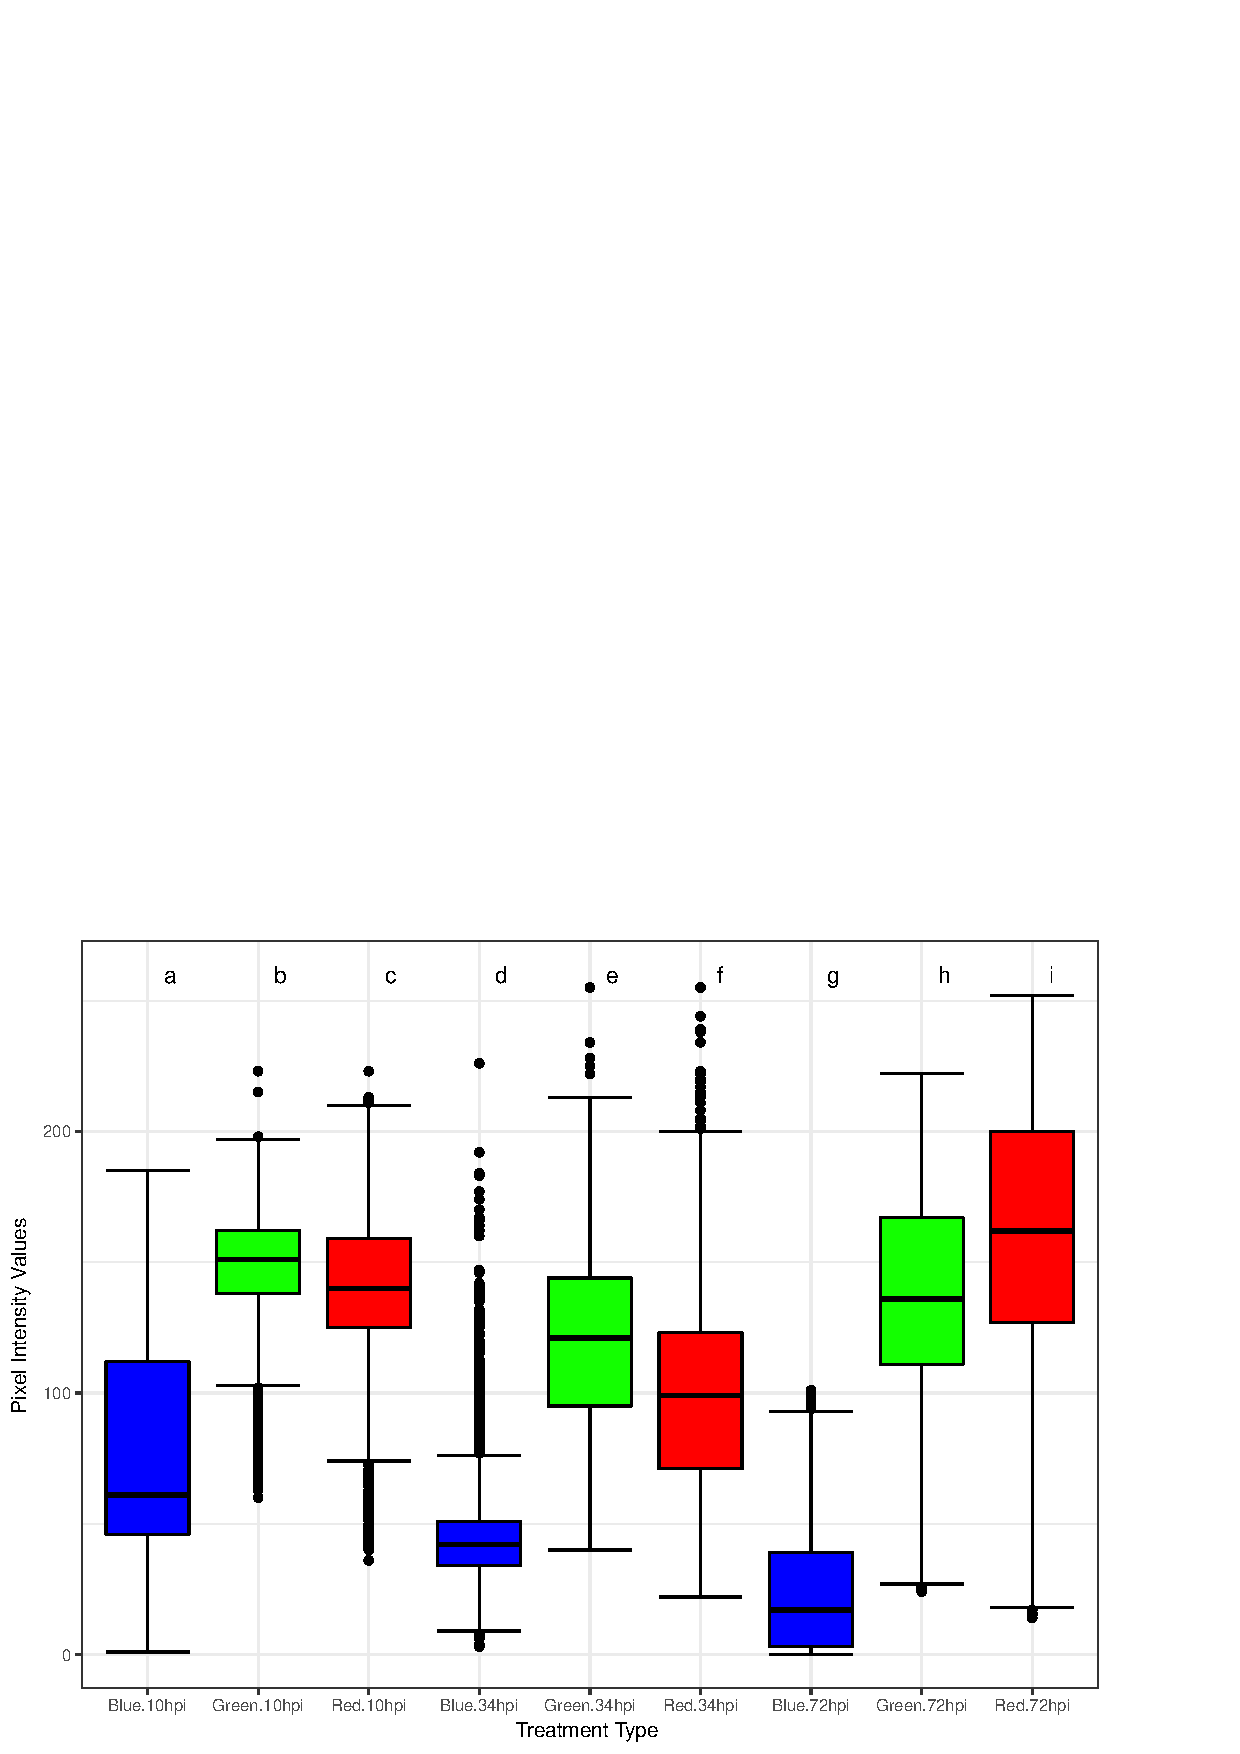
\includegraphics{treatments10.jpg}
\caption{True Positive test accuracy results for RF and CNN infection duration classifiers.}
\end{figure}

\begin{figure*}[!t]
\includegraphics{treatments202.jpg}
\caption{True Positive test accuracy results for RF and CNN treatment classifiers.}
\end{figure*}


\begin{figure*}[!b]
\includegraphics[height = 16cm]{CNN_rot.jpg}
\caption{Layout of the CNN used.}
\end{figure*}

\end{document}
